
\documentclass[11pt]{beamer}
\usetheme{Frankfurt}
\usecolortheme{seahorse}
\usepackage{multirow}
\usepackage{pifont}
\usepackage{bm}
\usepackage{caption}
%\usepackage{subcaption}
\usepackage{url}


\setbeamertemplate{footline}[frame number]
\setbeamertemplate{itemize items}[triangle]
\setbeamertemplate{frametitle}[default][center]




% Symbols
\newcommand{\ra}{\rightarrow}
\newcommand{\ov}{\overline}
\newcommand{\ur}{\underline}
\newcommand{\pr}{\prime}
\newcommand{\tbf}{\textbf}
\newcommand{\omg}{\Omega}
\newcommand{\mc}{\mathcal}
\newcommand{\lt}{\left}
\newcommand{\rt}{\right}
\newcommand{\mb}{\mathbb}
\newcommand{\imp}{\implies}
\newcommand{\dimp}{\Leftrightarrow}
\newcommand{\wh}{\widehat}
\newcommand{\dg}{\mc{D}}


% Sets
\newcommand{\realset}{\mb{R}}
\newcommand{\comprealset}{\mb{\ov{R}}}
\newcommand{\pint}{\mb{Z}_{> 0}}
\newcommand{\nzrl}{\mb{R}_{\geq 0}}
\newcommand{\prl}{\mb{R}_{>0}}
\newcommand{\rl}{\mb{R}}
\newcommand{\fin}{\forall i\in\{1,...,n\}}
\newcommand{\tup}[1]{\{1,...,#1\}}
\newcommand{\seq}[2]{_{#1=1}^#2}
\newcommand{\mCnn}{\mb{M}_{n\times n}(\mb{C})}
\newcommand{\mCmm}{\mb{M}_{m\times m}(\mb{C})}
\newcommand{\mCpn}{\mb{M}_{p\times n}(\mb{C})}
\newcommand{\mCnm}{\mb{M}_{n\times m}(\mb{C})}
\newcommand{\mRnn}{\mb{M}_{n\times n}(\mb{R})}
\newcommand{\mRpn}{\mb{M}_{p\times n}(\mb{R})}
\newcommand{\mRnm}{\mb{M}_{n\times m}(\mb{R})}
\newcommand{\mRno}{{{\mb{R}}}^n_{\geq 0}}
\newcommand{\mRmo}{{{\mb{R}}}^m_{\geq 0}}
\newcommand{\mRo}{\mb{R}_{\geq 0}}
\newcommand{\mRn}{{\mb{R}}^n}
\newcommand{\mRm}{{\mb{R}}^m}
\newcommand{\mCn}{\mb{C}^n}
\newcommand{\mCm}{\mb{C}^m}
\newcommand{\inv}{\mb{GL}_n(\mb{R})}
\newcommand{\id}[1]{\mb{I}_{#1\times #1}}
\newcommand{\mat}[3]{\mb{M}_{#1\times #2}(\mb{#3})}


% matrix operations
\newcommand{\ColumnJoin}[2]{\left[\begin{array}{l}{#1}\\{#2} \end{array}\right]}
\newcommand{\minaffine}[2]{\Lambda^{\min}\lt(#1,#2\rt)}
\newcommand{\maxaffine}[2]{\Lambda^{\max}\lt(#1,#2\rt)}

% local macros
\DeclareMathOperator{\real}{\operatorname{Re}}
\newcommand{\CZ}{\lt(V,c,s\rt)}
\newcommand{\GCZ}{\gcz{V}{c}{s}{W}{l}{u}}
\newcommand{\cz}[3]{\mc{C}\lt(#1,#2,#3\rt)}
\newcommand{\CZO}{\lt(V,0,s\rt)}
\newcommand{\czo}[2]{\mc{Z}\lt(#1,0,#2\rt)}
\newcommand{\trj}[2]{{\bf #1}(#2)}
\newcommand{\IncTcz}[6]{\mc{T}\lt(#1,#2,#3,#4,#5,#6\rt)}
\newcommand{\IncGcz}[6]{\mc{G}\lt(#1,#2,#3,#4,#5,#6\rt)}
\newcommand{\Ptope}[3]{\mc{P}\left(#1,#2,#3\right)}
\newcommand{\gcz}[6]{\mathcal{Z}\lt(#1,#2,#3,#4,#5,#6\rt)}
\newcommand{\sptope}[3]{\mathcal{P}\lt(#1,#2,#3\rt)}
\newcommand{\system}{\mb{H}}
\newcommand{\locationset}{Q}
\newcommand{\edgeset}{E}
\newcommand{\stay}{\gamma}
\newcommand{\linearmapset}{\mc{A}}
\newcommand{\inputset}{U}
\newcommand{\initialset}{\Omega}
\newcommand{\edge}{\sigma}
\newcommand{\loc}{q}
\newcommand{\map}{\linearmapset}
\newcommand{\inp}{\inputset}
\newcommand{\ptemplate}{\mc{K}}
\newcommand{\systrj}[2]{\lt({\bf #1},{\bf #2}\rt)}
\newcommand{\wholenums}{\mb{Z}_\geq 0}
\newcommand{\preloc}[1]{#1_{1}}
\newcommand{\postloc}[1]{#1_{2}}
\newcommand{\upperedgebound}[1]{#1^+}
\newcommand{\loweredgebound}[1]{#1^-}
\newcommand{\reset}[1]{#1_r}
\newcommand{\locationtransition}[1]{R_{#1}}
\newcommand{\edgetransition}[1]{R_{#1}}
\newcommand{\staysptope}[1]{\sptope{\ptemplate\lt(#1\rt)}{\stay^-\lt(#1\rt)}{\stay^+\lt(#1\rt)}}
\newcommand{\guardsptope}[1]{\sptope{\ptemplate\lt(\preloc{#1}\rt)}{\max\lt(\loweredgebound{#1},\stay^-\lt(\preloc{#1}\rt)\rt)}{\min\lt(\upperedgebound{#1},\stay^+\lt(\preloc{#1}\rt) \rt)}}
\newcommand{\hybridset}{\Gamma}
\newcommand{\transfer}[4]{#1#4 = #2\dg\lt(#3\rt)}
\newcommand{\centertransfer}[4]{#1#4 = #3-#2}
\newcommand{\scalebound}[5]{\max_{i=1}^{#4}\lt(\lt(\sum_{j=1}^{#5}\lt|#1\rt|_j\rt)-#3_i+#2_i\rt)}
\newcommand{\pseudoinverse}[1]{#1\lt(#1#1^T\rt)^{-1}}


\title{Augmented Complex Zonotopes for Computing Invariants of Affine Hybrid Systems}
\setbeamercolor{author}{fg=blue}
\author[shortname]{{ \bf \hspace{-1em} Arvind\ Adimoolam~\inst{1}\hspace{1em} Thao\ Dang~\inst{2}}}
\setbeamercolor{institute}{fg=blue}
\institute{{\bf
\inst{1,2} VERIMAG/ \inst{2}CNRS}\\~Grenoble,France
\begin{figure}
\center
\hspace{2em}
\includegraphics[scale=0.2]{fig/LogoVERIMAG.png}
\end{figure}
}

\date{}

\begin{document}

\maketitle

\begin{frame}{Hybrid behavior of digital control systems}
\textcol{Switch} between \textcol{different control laws}.\\
Eg.  \textcol{Different dynamics} of an engine for \textcol{different gears}.
\begin{figure}
\center
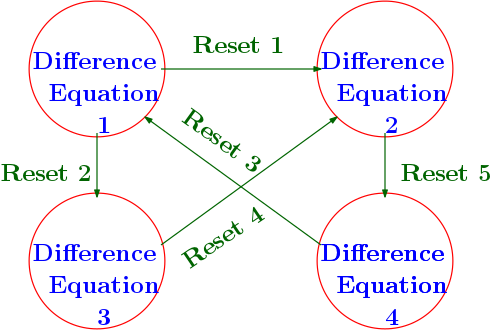
\includegraphics[scale=0.4]{fig/hybrid-model.png}
\end{figure}
\begin{itemize}
\item Difference Equation: $x(t+1)=f_i\lt(x(t),u(t)\rt).$
\item Reset: \vspace{-1.5em}
\begin{align}
\begin{split}
& \text{If}~~x\in S~~\text{(Precondition)}\\
& \text{then}~~x = g_i(x)
\end{split}
\end{align}
\end{itemize}
\end{frame}

\begin{frame}{Affine hybrid system}
%\begin{minipage}[t][0.3\textheight][t]{\textwidth}
\begin{figure}
\center
{\bf Specification}
\end{figure}
\begin{figure}
\center
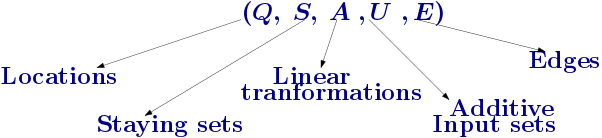
\includegraphics[scale=0.35]{fig/model-spec.png}
\caption*{{\small{\color{darkgray}$\forall q\in Q$, $S_q, U_q$: Polytopic subsets of $\realset^n$, $A_q: n\times n$ Real matrix.
$\forall \sigma\in E$: $\sigma = \lt(\sigma^-,\sigma^+,G_\sigma,A_\sigma,U_\sigma\rt)$, $\sigma^-\in Q$: Pre-location, $\sigma^+\in Q$: Post-location,
$G_\sigma$: Guard set $=>$ Polytopic subset of $\realset^n$, $A_\sigma: n\times n$ Real matrix, $U_\sigma$: Polytopic subsets of $\realset^n$}}}
\end{figure}
%\end{minipage}
\hrule
\begin{figure}
\center
{\bf Dynamics}
\end{figure}
\begin{minipage}{0.45\textwidth}
\begin{figure}
\centering
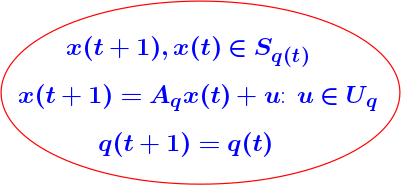
\includegraphics[scale=0.35]{fig/cont-transition.png}
\caption*{{\color{black}\hspace{1em} Continuous transition}}
\end{figure}
\end{minipage}
\hspace{1em}\vrule\hspace{1em}
\begin{minipage}{0.45\textwidth}
\begin{figure}
\centering
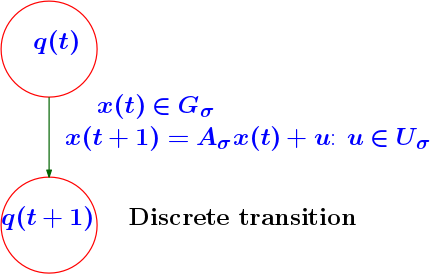
\includegraphics[scale=0.33]{fig/dis-transition.png}
\end{figure}
\end{minipage}
\end{frame}

\begin{frame}{Positive Invariant}
\begin{overprint}
\only<1>{
\begin{figure}
\center
\caption*{{\large \eqncol{$P$: Positive Invariant $\Leftrightarrow$ $\forall x(t)\in P:~ x(t+1)\in P$}}}
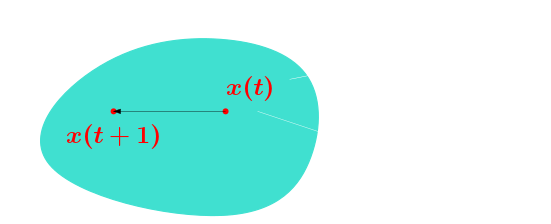
\includegraphics[scale=0.4]{fig/PosInv1.png}
\end{figure}
}
\only<2>{
\begin{figure}
\center
\caption*{{\large \eqncol{$P$: Positive Invariant $\Leftrightarrow$ $\forall x(t)\in P:~ x(t+1)\in P$}}}
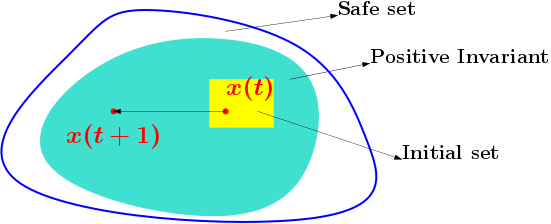
\includegraphics[scale=0.4]{fig/PosInv.png}
\end{figure}
}
\pause
\begin{itemize}
\item (\textcol{Initial set} \eqncol{$\subseteq$} \textcol{Positive Invariant} \eqncol{$\subseteq$} \textcol{Safe Set}) \eqncol{$\Leftrightarrow$} \textcol{System is safe}.
\item Useful for \textcol{Proving Safety Properties}, finding \textcol{ Safe Initial Conditions}.
\end{itemize}
\end{overprint}
\end{frame}

\begin{frame}{Set Representations for Computing Positive Invariants}
\begin{itemize}
\item Computing Smallest {\color{red} Positive Invariant} generally involves { \color{red} Iterative Unions} whose {\color{red}Convergence can be very Slow}\pause
\item Use \textcol{Specific set representations} to \textcol{Accelerate convergence}.\\
{\color{brown} Examples}
\begin{enumerate}
\item \textcol{Polytopes} $\Rightarrow$ Use \textcol{Convex Hull} overapproximation~\cite{todo}.
\item \textcol{Ellipsoids} $\Rightarrow$ solve \textcol{Linear Matrix Inequalities}.
\item \textcol{Template Linear inequalities} \cite{todo} and \textcol{Quadratic Inequalities} \cite{todo} \\$\Rightarrow$ Use \textcol{ Widening} or \textcol{Policy Iteration}.
\end{enumerate}
\end{itemize}
\end{frame}

\begin{frame}{Features of a good set representation}
\begin{enumerate}
\item \textcol{Guaranteed Existence of invariant} in the \textcol{linear case}.\\
{\color{brown} For example}
\begin{itemize}
\item \textcol{Elliposidal invariants} for linear system exist and computed easily by \textcol{LMI or eigenstructure}.
\item But \eqncol{Polyhedral invariants} can have \eqncol{Very Large Number of Faces}, hence sometimes \eqncol{Computationally Expensive}.
\end{itemize}
\item \textcol{Efficient computation/approximation} of system operations, like \textcol{Minkowski sum, linear transformation}, etc.\\
{\color{brown} For example}
\begin{itemize}
\item \textcol{Zonotopes}~\cite{todo}$\subseteq$ {\color{brown} Polyhedra}, \textcol{closed and efficient to compute}  \textcol{Minkowski sums and Linear transformations}.
\item \eqncol{Ellipsoids} - \eqncol{Not good for approximating Minkowski sums}
\begin{figure}

\includegraphics[scale=0.3]{fig/minkowski-ellipsoid.png}
\end{figure}
\end{itemize}
\end{enumerate}
\end{frame}

\begin{frame}{Template Complex Zonotope}
\eqncol{Extension} of \eqncol{Simple/Real zonotope} to \eqncol{Complex Numbers} to incorporate \eqncol{Complex Eigenstructure} of systems.\cite{todo}
\begin{overprint}
\only<1,2>{
\begin{exampleblock}{Simple/Real Zonotope}
Let $W\in\mat{n}{k}{\mb{R}}$ and $l,u\in\mb{R}^m: l\leq u$.  Then 
 a \emph{real zonotope} is
{\color{teal}\bm{$\zon{W}{l}{u} = \lt\{W\zeta: \zeta\in\mb{R}^k,~\zeta_i\in[l_i,u_i]~\forall i\in \tup{k}\rt\}}.$}
\end{exampleblock}
}
\onslide<1,2>{
\begin{block}{Template complex zonotope}
Let $V\in\mat{n}{m}{\mb{C}}$ (template) and $s\in\mb{R}^m_{\geq 0}$ (scaling factors) and
$c\in\realset^n$ (center).  Then the following is a template complex zonotope:
\textcol{$\bm{\cz{V}{c}{s} =
\lt\{c+V\epsilon:\epsilon\in\mb{C}^m,~\lt|\epsilon_i\rt|\leq s_i~\forall
i\in\tup{m}\rt\}}.$}
\end{block}
}
\onslide<2>{
\begin{alertblock}{Advantages}
\begin{itemize}
\item \textcol{Guaranteed existence of invariant} in \textcol{linear case} based on \textcol{Complex Eigenstructure}.
\item \textcol{Closed} under \textcol{Minkowski sums and linear transformations.}
\end{itemize}
\end{alertblock}
}
\end{overprint}
\end{frame}


\begin{frame}{Geometric visualization}
\begin{minipage}{0.45\textwidth}
\begin{figure}
\caption*{\eqncol{Simple/Real zonotope: Minkowski sums of line segments}}
\hspace{-2em}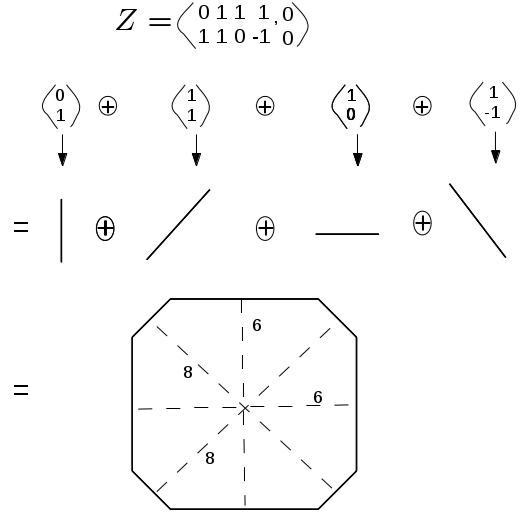
\includegraphics[scale=0.35]{fig/real-zonotope.png}
\end{figure}
\end{minipage}
\vrule
\hspace{1em}
\begin{minipage}{0.45\textwidth}
\begin{figure}
\caption*{\eqncol{Complex zonotope: Minkowski sums of line segments and some ellipsoids}}
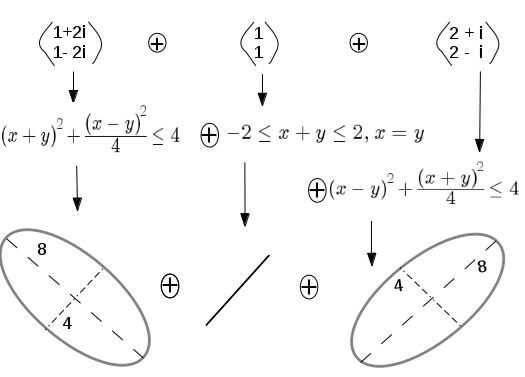
\includegraphics[scale=0.4]{fig/complex-zonotope.png}\\
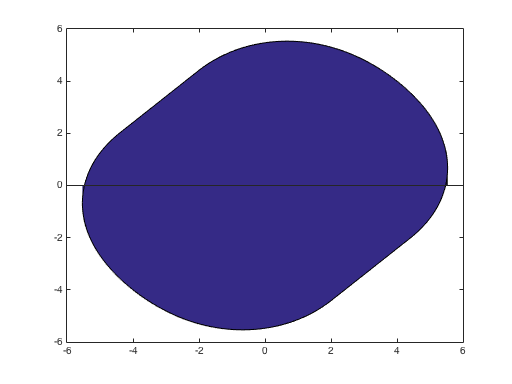
\includegraphics[scale=0.2]{fig/CZhull.png}
\end{figure}
\end{minipage}
\end{frame}


\begin{frame}{Guaranteed Existence of Invariant for Linear system}
Based on \textcol{{\bf Eigenstructure}} \\
Let $A\in\mat{n}{n}{R}$, then
\large{
\begin{block}{Proposition}
\center{
\begin{align*}
 A\cz{[e_1,...,e_n]}{0}{s}   = \cz{[e_1,...,e_n]}{0}{\dg\lt(\lt|\mu_i\rt|\rt)s}
\end{align*}
}
\end{block}
}
\center{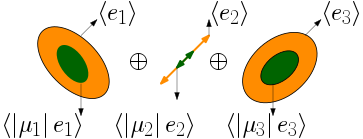
\includegraphics[scale=0.6]{fig/ContractionCZ.png}}
\end{frame}

\begin{frame}{Drawback of Simple and Template Complex Zonotopes}
\begin{itemize}
\item $\lt(\rt.$\textcol{Simple Zonotope} \eqncol{$\bigcap$} \textcol{Linear Constraints} (i.e. {\color{teal}$Tx\leq d$})$\lt.\rt)$\\ = (\eqncol{Polytope with exponential no. faces})
\eqncol{$\neq$ Zonotope}
\item $\lt(\rt.$\textcol{Complex Zonotope} \eqncol{$\bigcap$} \textcol{Linear Constraints} (i.e. {\color{teal}$Tx\leq d$})$\lt.\rt)$\\= (\eqncol{Non-polyhedral set})
\eqncol{$\neq$ Complex Zonotope}
\end{itemize}
{\color{violet}{\bf However!}}
\begin{exampleblock}{Sub-parallelotope constraints}
Let $K\in\mat{k}{n}{R}$ such that $k\leq n$ and $\lt(KK^T\rt)$ is
non-singular.  Let
  $\wh{u},\wh{l}\in\comprealset^k$ such that $\wh{l}\leq\wh{u}$.  Then
  a sub-parallelotopic set is $\sptope{K}{\wh{l}}{\wh{u}} = \lt\{x\in\realset^n: \wh{l}\leq Kx \leq \wh{u}\rt\}$.
\end{exampleblock}
\begin{block}{Observation: Intersection with alligned sub-parallelotope}
\textcol{\[\bm{
\zon{\pinv{K}}{l}{u} \bigcap \sptope{K}{\wh{l}}{\wh{u}}
= \zon{\pinv{K}}{l\bigvee \wh{l}}{u\bigwedge \wh{u}}}
\]}
\end{block}
\end{frame}

\begin{frame}{Augmented Complex Zonotope}
\textcol{Minkowski sum} of \textcol{Complex Zonotope} and \textcol{Real Zonotope}.
\begin{definition}
Let $V\in\mat{n}{m}{C}$ \eqncol{(primary template)}, $W\in\mat{n}{k}{R}$
\eqncol{(secondary template)}, $c\in\mb{R}^n$ \eqncol{(primary offset)},
$s\in\mb{R}^m$ \eqncol{(scaling factors)}, $u,l\in\mb{R}^k$ \eqncol{(lower
and upper interval bounds)} such that $l\leq u$.  
\begin{equation*}
\bm{\textcol{\gcz{V}{c}{s}{W}{l}{u} = \cz{V}{c}{s}\oplus\zon{W}{l}{u}}}.
\end{equation*}
\end{definition}
\end{frame}

\begin{frame}{Intersection with Sub-parallelotope}
\begin{exampleblock}{Affine approximation of multi-variable Min and Max functions}
{\small
\begin{itemize}
\item \textcol{Min-approximation function}:
$\lt(\minaffine{u}{\wh{u}}\rt)_i = \left\{
\begin{array}{l}
\wh{u}_i~~\text{if}~\wh{u}_i<\infty\\
u_i~~\text{if}~\wh{u}_i=\infty
\end{array}
\right..$\\
\item \textcol{Max-approximation function}:
$\lt(\maxaffine{l}{\wh{l}}\rt)_i = \left\{
\begin{array}{l}
\wh{l}_i~~\text{if}~\wh{l}_i>\infty\\
l_i~~\text{if}~\wh{l}_i=-\infty
\end{array}
\right..$
\end{itemize}
}
\end{exampleblock}
\begin{block}{Theorem: Affine overapproximation of Intersection with Sub-parallelotope}~\label{thm:acz-int}
{\small Given sub-parallelotope \textcol{$\sptope{\ptemplate}{\wh{l}}{\wh{u}}$},
augmented complex zonotope \textcol{$\gcz{V}{c}{s}{\pinv{\ptemplate}}{l}{u}$}
such that \eqncol{$V\conjtranspose{V}$ is non-singular, $\lt|\pinv{V}c\rt|\leq s$, $l\leq
\maxaffine{l}{\wh{l}}\leq \minaffine{u}{\wh{u}}\leq u$}:}
\vspace{-1em}
\textcol{
\begin{align*}
\begin{split}
&\bm{\gcz{V}{c}{s}{\pinv{\ptemplate}}{l}{u}\bigcap\sptope{\ptemplate}{\wh{l}}{\wh{u}}}
 \bm{\subseteq \gcz{V}{c}{s}{\pinv{\ptemplate}}{\maxaffine{l}{\wh{l}}}{\minaffine{u}{\wh{u}}}}
\end{split}
\end{align*}
}
\end{block}
%
\end{frame}

\begin{frame}{Minkowski sum and Linear Transformation}
\begin{block}{Closure under Linear transformation and Minkowski sum}
\begin{enumerate}
\item $A\gcz{V}{c}{s}{W}{l}{u} = \gcz{AV}{Ac}{s}{AW}{l}{u}$.
\item $~$\vspace{-2em}\hspace{-2em}\begin{align*}
&\gcz{V}{c}{s}{W}{l}{u}\oplus\gcz{V^\pr}{c^\pr}{s^\pr}{W^\pr}{l^\pr}{u^\pr}\\
&= \gcz{\lt[V~V^\pr\rt]}{c+c^\pr}{\ColumnJoin{s}{s^\pr}}{\lt[W~W^\pr\rt]}{\ColumnJoin{l}{l^\pr}}{\ColumnJoin{u}{u^\pr}}.
\end{align*}
\end{enumerate}
\end{block}
%
\begin{alertblock}{}
\begin{itemize}
\item For \eqncol{fixed primary and secondary templates} of augmented complex zonotopes, {\bf Linear transformation and Minkowski sums} of are \textcol{Affine functions of rest variables}.
\end{itemize}
\end{alertblock}
\end{frame}
%
\begin{frame}{Inclusion between Template Complex Zonotopes}
Let \textcol{$\cz{V^\pr_{n\times
    m^\pr}}{c^\pr}{s^\pr}\order \cz{V_{n\times m}}{c}{s}$} if
\eqncol{\begin{align*}~\label{eqn:tcz-inc}
\begin{split}
& \exists X\in\mat{m}{m^\pr}{\mb{C}}~\text{and}~y\in\mb{C}^{m}~\text{s.t.}\\
& \transfer{V}{V^\pr}{s^\pr}{X},~~~\centertransfer{V}{c}{c^\pr}{y},~\text{and}~
 \scalebound{X}{y}{s}{m}{m^\pr}\leq 0\\
\end{split}
\end{align*}
}
\textcol{Theorem}: \eqncol{$(\order)\implies(\subseteq)$} among \eqncol{Template Complex zonotopes}.
%
\begin{alertblock}{}
For fixed \eqncol{template}, \textcol{$\order$} defines \textcol{SOCC (convex constraints) on rest variables}.
\end{alertblock}
\end{frame}
%
\begin{frame}{Real Inclusion between Augmented Complex Zonotopes}
\begin{block}{}
Let \textcol{$\gcz{V^\pr}{c^\pr}{s^\pr}{W^\pr}{l^\pr}{u^\pr}\order
\gcz{V}{c}{s}{W}{l}{u}$} if\\ \eqncol{$\cz{\lt[V^\pr~W^\pr\rt]}{c^\pr+W^\pr\lt(\frac{u^\pr+l^\pr}{2}\rt)}{\ColumnJoin{s^\pr}{\frac{u-l}{2}}}
\order
\cz{\lt[V~W\rt]}{c+W\lt(\frac{u+l}{2}\rt)}{\ColumnJoin{s}{\frac{u-l}{2}}}$}\\
\end{block}
\textcol{Theorem}: \eqncol{$(\order)\implies(\subseteq)$} among \eqncol{Real Projections of Augmented Complex zonotopes}.
\begin{alertblock}{}
For fixed \eqncol{primary and secondary templates}, \textcol{$\order$} defines \textcol{SOCC (convex constraints) on rest variables}.
\end{alertblock}
\end{frame}
%
\begin{frame}{Inclusion inside Polytopic safe set}
Consider a \eqncol{Safe set} defined by a \eqncol{Polytope $S=Tx\leq d$}.  Then \eqncol{$\real\lt(\gcz{V}{c}{s}{W}{l}{u}\rt)\subseteq S$} if
%
\begin{block}{}
\textcol{
\[
T\lt(c+W\lt(\frac{u+l}{2}\rt)\rt)+\lt|T\lt[V,~\pinv{\ptemplate}\rt]\rt|\begin{bmatrix}s\\ \frac{u-l}{2}\end{bmatrix}\leq d.
\]
}
\end{block}
%
\begin{alertblock}{}
For fixed \eqncol{primary and secondary templates}, the above inequality defines \textcol{SOCC (convex constraints) on rest variables}.
\end{alertblock}
\end{frame}


\begin{frame}{Convex Program for Computing Positive Invariant}
\begin{overprint}
\only<1>{\begin{exampleblock}{Assumptions}
\begin{enumerate}
\item Let \eqncol{Guards and Staying sets of Hybrid system} be specified by
\textcol{Sub-parallelotopes with common template} {\color{violet}(can model many real-world examples).}
\item {\color{violet} Fix primary and Secondary templates} of
augmented complex zonotopes, so, 
\textcol{Variables := primary offsets, scaling factors, lower and
upper interval bounds}.
\end{enumerate}
\end{exampleblock}
}
\onslide<1,2>{
\begin{block}{Recap}
\begin{itemize}
\item \eqncol{Linear Transformation and Minkowski sum} - \textcol{Affine function}
\item \eqncol{Overapproximation of Intersection with
Sub-parallelotopic constraints when aligned} - \textcol{Affine function}
\item \eqncol{Inclusion between Augmented Complex Zonotopes (sufficient condition)} - \textcol{SOCC (convex) constraints}
\item \eqncol{Inclusion inside Polytopic (Safe) set} - \textcol{Linear  constraints}
\end{itemize}
\end{block}
}
\pause
\begin{alertblock}{Result}
{Using above, we can derive \textcol{\bf Second order conic (convex)
constraints} in
above variables to compute \textcol{Positive Invariant} inside
a \textcol{Safe set} containing  an \textcol{Initial zonotopic set!}}
\end{alertblock}
\end{overprint}
\end{frame}

\begin{frame}{Choosing Templates}
\begin{itemize}
\item \textcol{Secondary template} is fixed as \textcol{Pseudo-Inverse} of system \textcol{Sub-Parallelotopic template}.\pause
\end{itemize}
\begin{block}{Chosing Primary Template}
All or some of the following:\pause
\begin{enumerate}
\item Eigenvectors of the transformation matrices and their products, for
   the different transition maps.  \pause  
\item  The primary and
   secondary templates of the zonotopes which overapproximate the
   additive disturbance input sets and their products with the linear
   matrices of the transition maps.  \pause
\item
   Orthogonal projections of the above vectors on the null space of
   the subparallelotopic template.  \pause
\item Adding any set of arbitrary vectors will increase the
   chance of computing a desired invariant, but at a computational
   expense.  This is because the scaling factors will be adjusted
   accordingly by the optimizer.
\end{enumerate}
\end{block}
\end{frame}

\begin{frame}{Example 1: NXT-Lego Robot model}
\eqncol{Benchmark example} published in \eqncol{ARCH 2014~\cite{heinz2014benchmark}} \textcol{(Heinz, Oehlerking and Woehrle.)}

\begin{minipage}{0.3\textwidth}
\begin{figure}
\centering
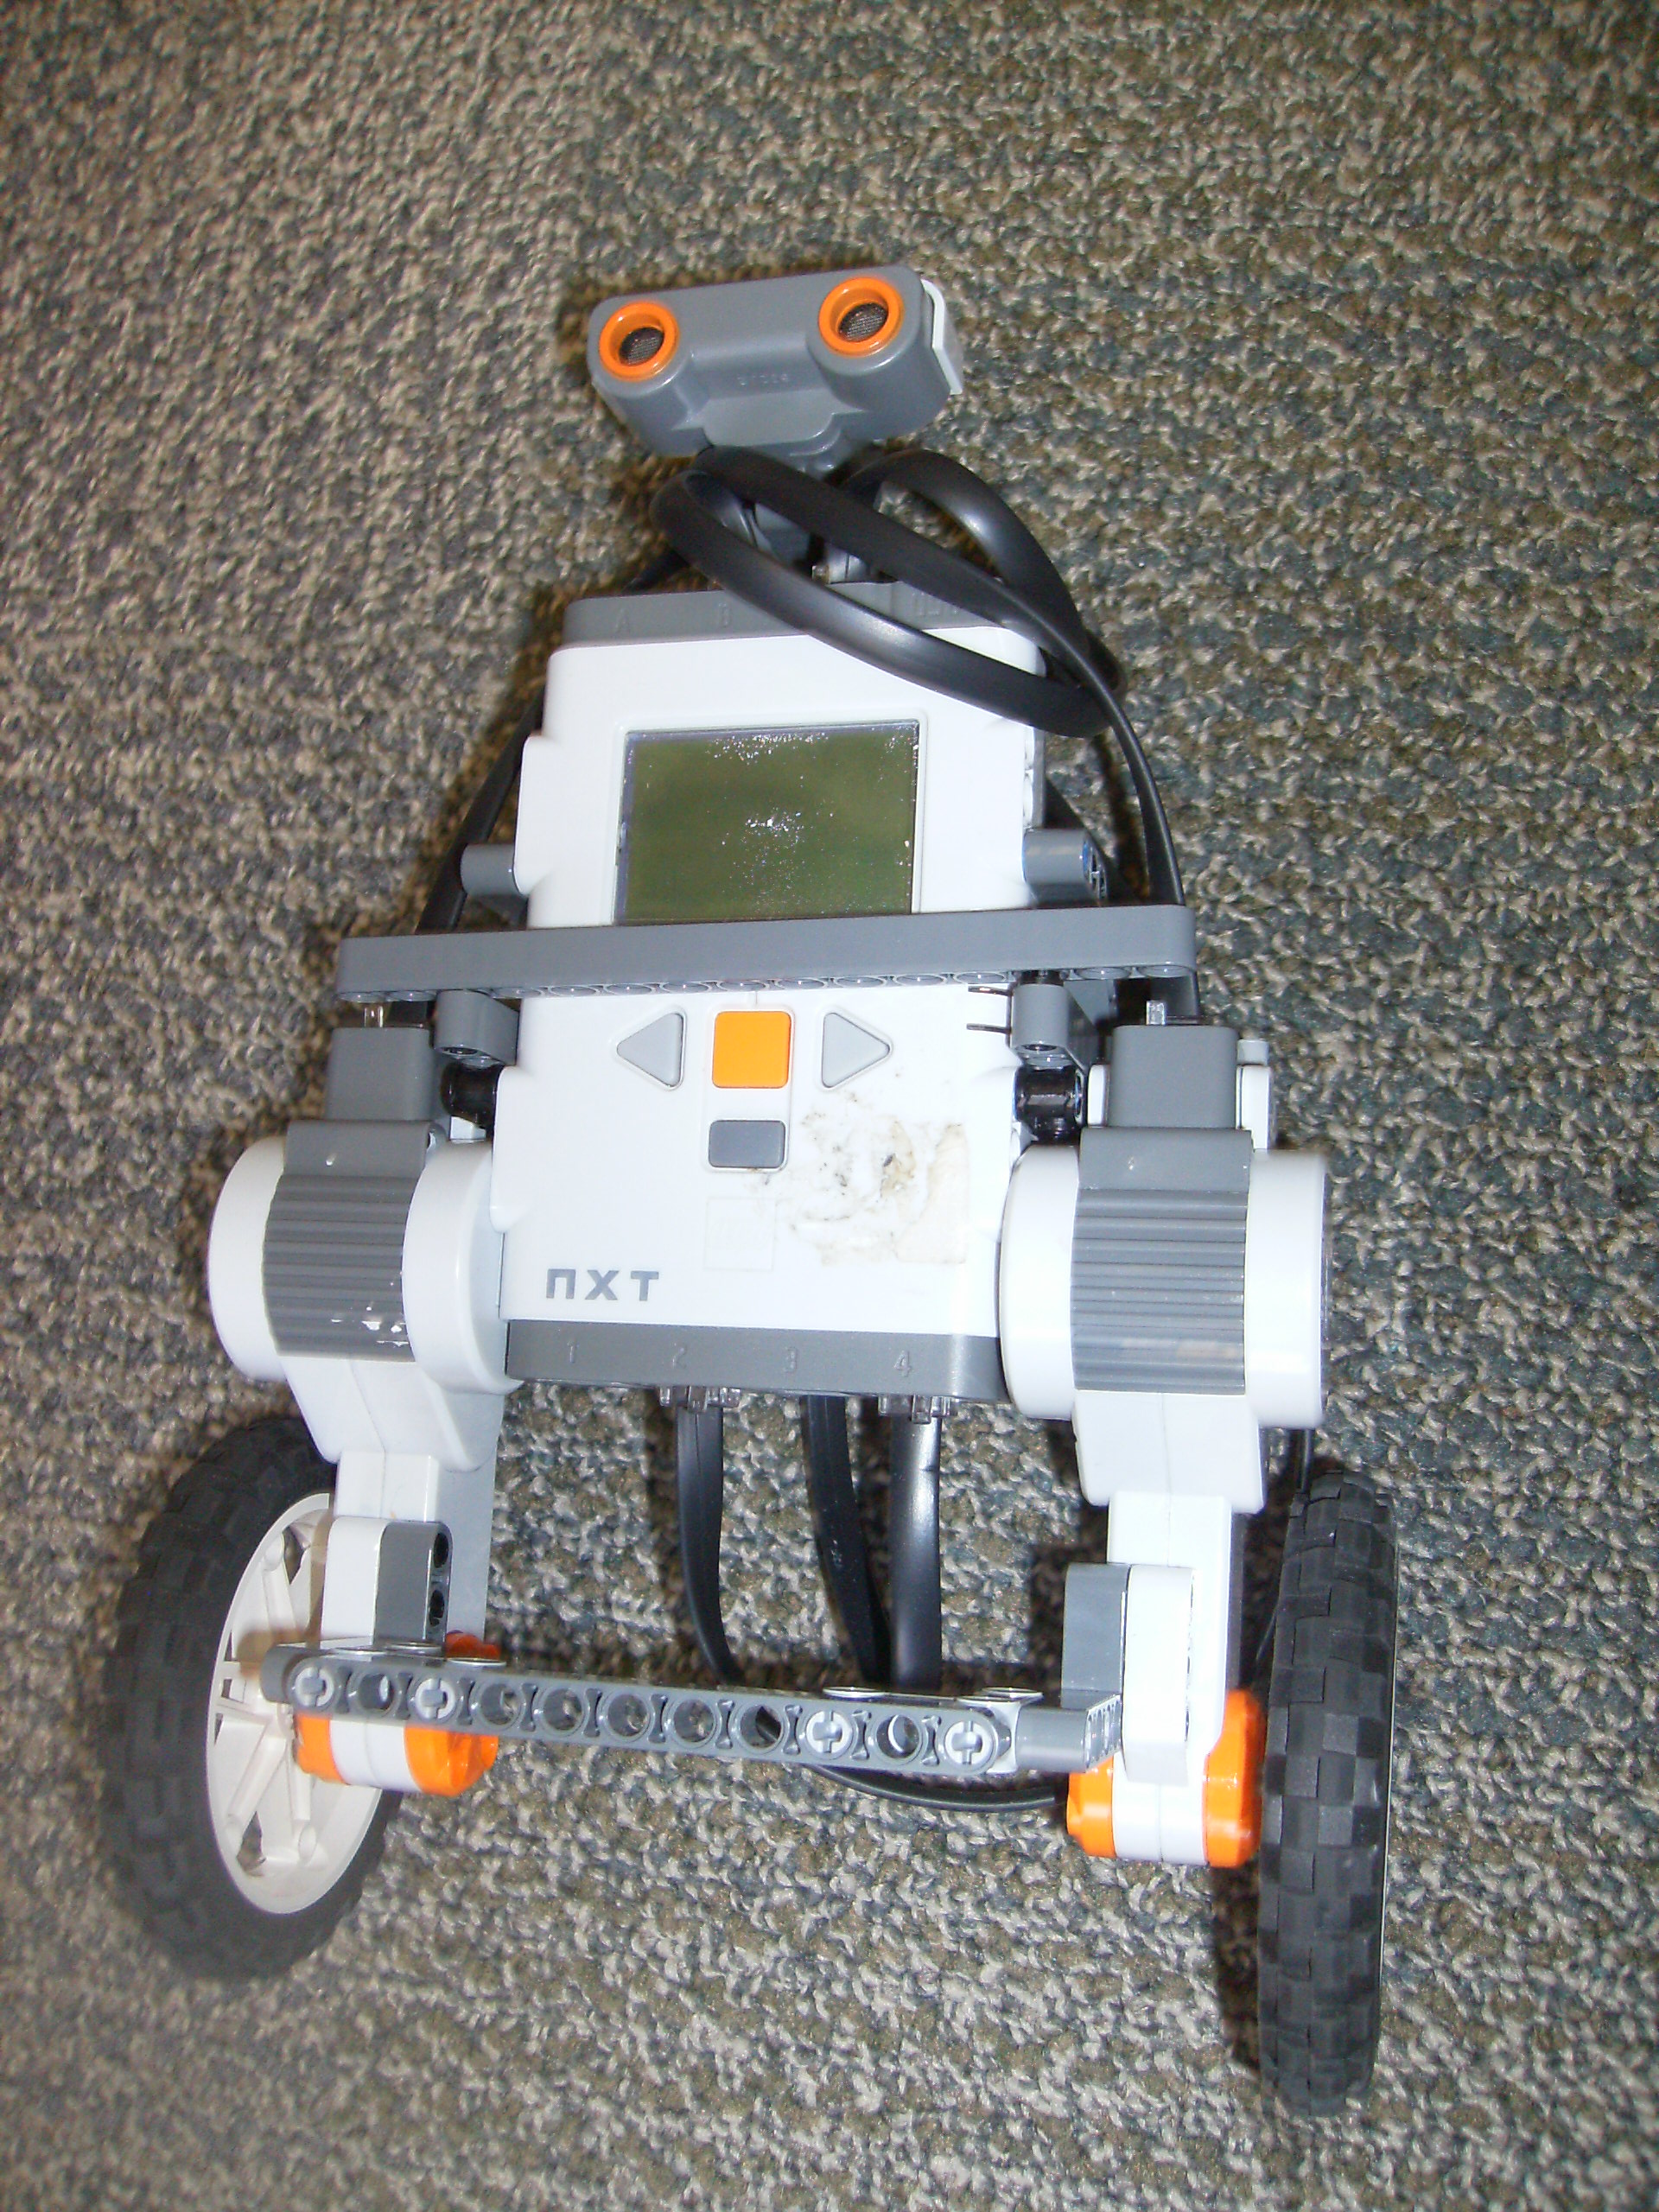
\includegraphics[scale=0.09]{fig/NXT-lego.JPG}
\end{figure}
\end{minipage}
\begin{minipage}{0.6\textwidth}
{\footnotesize Lego NXT self-balancing robot by\\ Medelen8/CC-BY-SA-3.0}
\begin{itemize}
\item \textcol{Sampled data Networked Control System}: Controller input to Plant sampled at discrete time instants.
\item Input from controller has \textcol{saturation} on {\color{violet} 2 controller inputs}: \textcol{Hybrid behavior}.
\end{itemize}
\end{minipage}

\eqncol{After transformation to decouple unbounded directions, we obtained}\\
%% \begin{block}{}
%% $
%% \lt[\begin{array}{cc}\trj{x}{t+1} &
%%     \trj{y}{t+1}\end{array}\rt]^T=F_1\trj{x}{t}+F_2sat\lt(\trj{y}{t}\rt)+F_3\trj{u}{t}$\\
%% \textcol{Saturated}: $sat\lt(y_i\rt) = max\lt(-\delta
%% d_p,min\lt(y_i,\delta d_p\rt)\rt),~\forall i\in\{1,2\}$, where $\delta=100$
%% and $d_p=0.0807$. \textcol{Unsaturated}: $sat\lt(y_i\rt) = y_i$
%% \end{block}
\begin{block}{Complexity}
\begin{itemize}
\item \eqncol{Saturated}: \textcol{9 dimensional, 1 location, 9 edges.}
\item \eqncol{Unsaturated}: \textcol{9 dimensional linear system.}
\end{itemize}
\end{block}
\end{frame}

\begin{frame}{Verification challege: NXT-Lego Robot model}
\begin{alertblock}{Task}
Find/Verify bounds on \textcol{body pitch angle}.
\end{alertblock}
\begin{overprint}
\only<2>{
\begin{exampleblock}{Experimental settings}
\begin{itemize}
\item \eqncol{Primary template:}  (Complex) \textcol{Eigenvectors} of linear maps and their products,
 \textcol{Orthonormal
vectors} to guarding hyperplane normals.  For
the linear system, it consists of the eigenvectors of the linear map,
the \textcol{uncertain input set template} and its multiplication by the linear matrix
(related to affine map) and square of the linear matrix. 
\item \eqncol{SpaceEx settings:}  \textcol{Octagon template} and a
template with \textcol{$400$ uniformly sampled support vectors}.
\end{itemize}
\end{exampleblock}
}
\end{overprint}
\end{frame}

\begin{frame}{Results: NXT-Lego Robot model}
\center{{\eqncol{\small{\footnotesize UB: $>$1000, ~~NT: Not terminating in more than 180s, \newline
  n/a: Not applicable/not available, ~~ACZ: Augmented complex
  zonotope.}}}}
{\color{black}
\begin{minipage}{0.48\textwidth}
\begin{table}
\centering
\resizebox{0.5\textheight}{0.35\textwidth}{
\begin{tabular}{|l|c|c|c|}
\hline
\multicolumn{2}{|c|}{\multirow{2}{*}{Method}} &
\multirow{2}{*}{$\lt|\psi\rt|\leq$} & Comp.\\
\multicolumn{2}{|c|}{} & & time (s)\\
\hline
\multirow{4}{*}{SpaceEx} & octagon & \multirow{2}{*}{UB} & \multirow{2}{*}{NT}\\
& template & & \\
\cline{2-4}
& 400 support & \multirow{2}{*}{UB} & \multirow{2}{*}{NT}\\
& vectors & &\\
\hline
\multicolumn{2}{|c|}{\multirow{2}{*}{Suggested in~\cite{heinz2014benchmark}}} &
\multirow{2}{*}{$1.39$} & \multirow{2}{*}{n/a}\\
\multicolumn{2}{|c|}{} & &\\
\hline
\multicolumn{2}{|c|}{\multirow{2}{*}{ACZ invariant}} & \multirow{2}{*}{$1.29$} &
\multirow{2}{*}{$4$}\\
\multicolumn{2}{|c|}{} & & \\
\hline
\end{tabular}
}
\caption*{{\footnotesize Unsaturated robot model: results}}
\end{table}
\end{minipage}
\begin{minipage}{0.48\textwidth}
\begin{table}
\centering
\resizebox{0.5\textheight}{0.35\textwidth}{
\begin{tabular}{|l|c|c|c|}
\hline
\multicolumn{2}{|c|}{\multirow{2}{*}{Method}} &
\multirow{2}{*}{$\lt|\psi\rt|\leq$} & Comp.\\
\multicolumn{2}{|c|}{} & & time (s)\\
\hline
\multirow{4}{*}{SpaceEx} & octagon & \multirow{2}{*}{UB} &
\multirow{2}{*}{NT}\\
& template & & \\
\cline{2-4}
& 400 support & \multirow{2}{*}{UB} & \multirow{2}{*}{NT}\\
& vectors & & \\
\hline
\multicolumn{2}{|c|}{\multirow{2}{*}{Suggested in~\cite{heinz2014benchmark}}} &
$1.571-\epsilon:$ & \multirow{2}{*}{n/a}\\
\multicolumn{2}{|c|}{} & $\epsilon>0$ &\\
\hline
\multicolumn{2}{|c|}{\multirow{2}{*}{ACZ invariant}} & \multirow{2}{*}{$1.13$} &
\multirow{2}{*}{45}\\
\multicolumn{2}{|c|}{} & &\\
\hline
\end{tabular}
}
\caption*{{\footnotesize Saturated robot model: results}}
\end{table}
\end{minipage}
}
\vspace{-2em}
\begin{alertblock}{Remarks}
\begin{itemize}
\item Model has \textcol{complex eigenstructure}, some eigenvalues have \textcol{magnitude close to 1}.
\item Since \textcol{Complex Zonotope uses complex eigenstructure}, where as \textcol{Polytope (SpaceEx)} \eqncol{can not use complex eigenstructure}.
\end{itemize}
\end{alertblock}
\end{frame}

\begin{frame}{Example 2: Perturbed double integrator}
\begin{itemize}
\item Example from \textcol{Rakovic et. al.-CDC 2004}~\cite{rakovic2004computation}.
\item \textcol{Piecewise affine with 2 dimensional additive disturbance input}, \eqncol{Four different Affine
dynamics} in \eqncol{Four different polytopic regions} of space.
\item Model complexity: \textcol{2 dimensions, 4 locations and 12 edges.}
\end{itemize}
\begin{alertblock}{Challenge}
\begin{enumerate}
\item Verify \textcol{smallest (possible) bounds} on the \textcol{two state space co-ordinates}.
\item Compute a \textcol{large set} of \textcol{safe initial conditions}.
\end{enumerate}
\end{alertblock}
\pause
\begin{exampleblock}{Experimental settings}
\begin{itemize}
\item  {\bf Primary template}: \textcol{Complex eigenvectors} of all linear matrices of the \textcol{affine maps and
their binary products}. 
\item  {\bf SpaceEx tool}: \eqncol{Two
different templates}: \textcol{Octagon} template and a template with \textcol{100
uniformly sampled support vectors}.
\end{itemize}
\end{exampleblock}
\end{frame}

\begin{frame}{Experimental results: PDI}
\begin{table}
\begin{minipage}{\textwidth}
\center
\caption*{Small invariant computation}
\begin{tabular}{|l|c|c|c|c|}
\hline
\multicolumn{2}{|c|}{\multirow{2}{*}{Method}} &
\multirow{2}{*}{$\lt|x_1\rt|\leq$} & \multirow{2}{*}{$\lt|x_2\rt|\leq$} & Comp.\\
\multicolumn{2}{|c|}{} & & & time (s) \\
\hline
\multirow{4}{*}{SpaceEx} & octagon & \multirow{2}{*}{0.38} &
\multirow{2}{*}{0.43} & \multirow{2}{*}{1.7}\\
& template & & &\\
\cline{2-5}
& 100 support & \multirow{2}{*}{0.38} & \multirow{2}{*}{0.43} & \multirow{2}{*}{23.6}\\
& vectors & & &\\
\hline
\multicolumn{2}{|c|}{\multirow{2}{*}{ACZ invariant}} &
\multirow{2}{*}{0.38} & \multirow{2}{*}{0.36} & 
\multirow{2}{*}{5.1}\\
\multicolumn{2}{|c|}{} & & &\\
\hline
\end{tabular}
\end{minipage}
\hspace{4em}
\begin{minipage}{\textwidth}
\center
\caption*{Large invariant computation}
\begin{tabular}{|c|c|}
\hline
\multirow{2}{*}{Method} & Comp.\\
& time (s)\\
\hline
\multirow{2}{*}{MPT tool~\cite{rakovic2004computation}} & \multirow{2}{*}{107}\\
& \\
\hline
\multirow{2}{*}{ACZ} & \multirow{2}{*}{12}\\
& \\
\hline
\end{tabular}
\end{minipage}
\end{table}
\end{frame}

\begin{frame}{Example 3: Networked vehicle platoon}
\begin{figure}
\caption*{\small Benchmark {\color{blue}  2014 ARCH Workshop}: \eqncol{Makhlouf and Kowalewski~\cite{makhlouf2014networked}}}
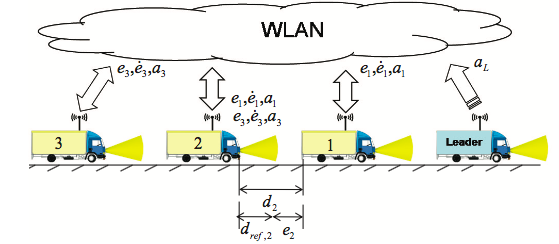
\includegraphics[scale=0.4]{fig/VehiclePlatoon.png}\\
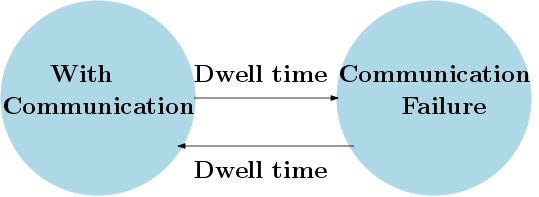
\includegraphics[scale=0.4]{fig/networked-platoon-model.png}
\end{figure}
\end{frame}

\begin{frame}{Verification challenge: Networked platoon}
\begin{alertblock}{Task}
\begin{itemize}
\item Find \textcol{minimum (possible) reference distances between vehicles} such that \eqncol{vehicles do not collide}.
\item Equivalent to finding \textcol{ upper bounds on $-e_1, -e_2$ and $-e_3$}.
\end{itemize}
\end{alertblock}
\pause
\begin{exampleblock}{Two cases}
\begin{enumerate}
\item \textcol{Slow switching}: \eqncol{Minimum dwell time 20 s}. {\color{violet} 9 dimensional, 2 locations, 4 edges}.
\item \textcol{Fast switching}: \eqncol{Integer dwell times}. {\color{violet} 9 dimensional, 2 locations, 2 edges}.
\end{enumerate}
\end{exampleblock}
\end{frame}

\begin{frame}{Expermimental results: Networked Platoon}
\begin{table}
\resizebox{1.1\textwidth}{!}{\hspace{-3em}
\begin{tabular}{|l|c|c|c|c|c|c|c|c|c|}
\hline
\multicolumn{2}{|c|}{\multirow{4}{*}{Method}} & \multicolumn{4}{|c|}{\multirow{2}{*}{Slow switching}} & \multicolumn{4}{|c|}{\multirow{2}{*}{Fast switching}}\\
\multicolumn{2}{|c|}{} & \multicolumn{4}{|c|}{} & \multicolumn{4}{|c|}{} \\
\cline{3-10}
\multicolumn{2}{|c|}{} & \multirow{2}{*}{$-e_1\leq$} & \multirow{2}{*}{$-e_2\leq$} & \multirow{2}{*}{$-e_3\leq$} & Comp. & \multirow{2}{*}{$-e_1\leq$} & \multirow{2}{*}{$-e_2\leq$} & \multirow{2}{*}{$-e_3\leq$} & Comp.\\
\multicolumn{2}{|c|}{} & & & & time (s) & & & & time (s)\\
\hline
\multirow{4}{*}{SpaceEx} & octagon & \multirow{2}{*}{28} &
\multirow{2}{*}{27} & \multirow{2}{*}{10} &
\multirow{2}{*}{NT} & \multirow{2}{*}{UB} &
\multirow{2}{*}{UB} & \multirow{2}{*}{UB} &
\multirow{2}{*}{NT}\\
& template & & & & & & & &\\
\cline{2-10}
& 100 support & \multirow{2}{*}{28} & \multirow{2}{*}{25} &
\multirow{2}{*}{13} & \multirow{2}{*}{1.3} & \multirow{2}{*}{UB} & \multirow{2}{*}{UB} &
\multirow{2}{*}{UB} & \multirow{2}{*}{NT}\\
& vectors & & & & & & & &\\
\hline
\multicolumn{2}{|c|}{\multirow{2}{*}{Real zonotope~\cite{makhlouf2014networked}}} &
\multirow{2}{*}{25} & \multirow{2}{*}{25} & \multirow{2}{*}{10}
 & \multirow{2}{*}{n/a} & \multirow{2}{*}{n/a} & \multirow{2}{*}{n/a} & \multirow{2}{*}{n/a}
 & \multirow{2}{*}{n/a}\\
\multicolumn{2}{|c|}{} & & & & & & & &\\
\hline
\multicolumn{2}{|c|}{\multirow{2}{*}{ACZ invariant}} &
\multirow{2}{*}{28} & \multirow{2}{*}{26} &
\multirow{2}{*}{12} & \multirow{2}{*}{12} &
\multirow{2}{*}{46} & \multirow{2}{*}{54} &
\multirow{2}{*}{57} & \multirow{2}{*}{12.6}\\
\multicolumn{2}{|c|}{} & & & & & & & &\\
\hline
\end{tabular}
}
%% \caption*{{\footnotesize UB: $>$1000, ~~NT: Not terminating in more than 180s, \newline
%%   n/a: Not applicable/not available, ~~ACZ: Augmented complex
%%   zonotope.
%% }}
\begin{alertblock}{Remarks}
\begin{itemize}
\item \eqncol{Slow switching model} is \textcol{more stable} than \eqncol{fast switching model}.
\item Since {\bf complex zonotope} used \textcol{eigenstructue}, it could also compute invariant for the \textcol{less stable: fast switching} model, while  {\bf Polytope (SpaceEx)} \eqncol{could not}.
\end{itemize}
\end{alertblock}
\end{table}
\end{frame}














\bibliographystyle{plain}
\bibliography{ref}



\end{document}
